\immediate\write18{tex hobby.dtx}
\documentclass{article}
\usepackage{amsmath}
\usepackage{pgfplots}
\usetikzlibrary{hobby,decorations.pathreplacing}
\usepackage[silent]{trace-pgfkeys}

\newif\ifhobbyinpath
\tikzset{
  tangent/.style={%
    called={tangent #1},
    in angle={(180+#1)},
    Hobby finish,
    Hobby action={\message{breaking path}},
    designated Hobby path=next,
    out angle=#1,
  },
  called/.code={\message{#1 got called}},
  every path/.append style={clear next Hobby path options,clear this Hobby path options},
  show curve controls/.style={
    decoration={
      show path construction,
      curveto code={
        \draw [blue, dashed]
        (\tikzinputsegmentfirst)    -- (\tikzinputsegmentsupporta)
        node [at end, draw, solid, red, inner sep=2pt]{};
        \draw [blue, dashed]
        (\tikzinputsegmentsupportb) -- (\tikzinputsegmentlast)
        node [at start, draw, solid, red, inner sep=2pt]{};
      }
    },decorate
  },
  Hobby externalise
}

\pgfmathparse{atan2(0,1)}
\show\pgfmathresult
\pgfmathparse{hobbyatan2(0,1)}
\show\pgfmathresult

\HobbyDisableAux

\begin{document}




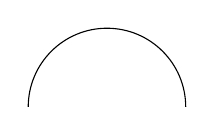
\begin{tikzpicture}[use quick Hobby shortcut]
\draw (0,0) .. (1,1) .. (2,0);
\end{tikzpicture}

\begin{tikzpicture}[use Hobby shortcut]
\draw[save Hobby path=temp] (0,0) .. (1,1) .. (2,0);
\tikzset{show Hobby path=temp}
\end{tikzpicture}

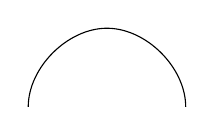
\begin{tikzpicture}
\draw (0,0) .. controls (0,.5) and (.5,1) .. (1,1) .. controls (1.5,1) and (2,.5) .. (2,0);
\end{tikzpicture}

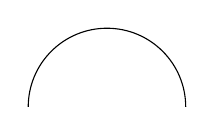
\begin{tikzpicture}
\draw (0,0) to[curve through={(1,1)}] (2,0);
\end{tikzpicture}


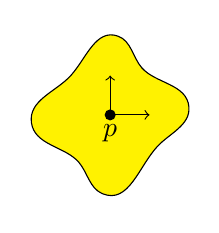
\begin{tikzpicture}[use Hobby shortcut,baseline=0pt]
\filldraw[fill=yellow] ([closed]1,0.1) .. (.4,.6) .. (0.1,1) .. (-.5,.5) .. (-1,-0.1) .. (-.4,-.6) .. (-.1,-1) .. (.6,-.4) .. (1,0.1);
\draw[->] (0,0) -- (0,.5);
\draw[->] (0,0) -- (.5,0);
\fill (0,0) circle[radius=2pt] node[below] {\(p\)};
\end{tikzpicture}

%\pgfmathsetseed{2}
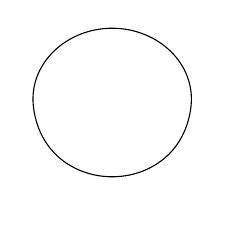
\begin{tikzpicture}
\draw[use Hobby shortcut] ([closed]0,0) .. (1,1) .. (2,0);
\end{tikzpicture}

\begin{tikzpicture}
\draw[use Hobby shortcut] (0:rnd+2) \foreach \ang in {0,20,...,350} { .. (\ang:rnd+2) };
\end{tikzpicture}

\begin{tikzpicture}
\draw[use Hobby shortcut] ([closed]0:rnd+2) \foreach \ang in {0,20,...,350} { .. (\ang:rnd+2) };
\end{tikzpicture}

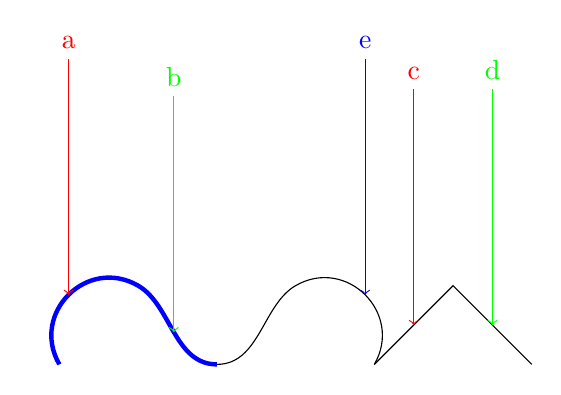
\begin{tikzpicture}[use Hobby shortcut]
\draw[save Hobby path={first}]
(1,0) .. coordinate (a) ([blank=soft]2,1) .. coordinate (b) ([blank=soft]3,0) .. (4,1) .. coordinate (e) (5,0);
\draw[ultra thick,blue,restore and use Hobby path={first}{disjoint,invert soft blanks}];
\draw[red,<-] (a) -- +(0,3) node[above] {a};
\draw[green,<-] (b) -- +(0,3) node[above] {b};
\draw[blue,<-] (e) -- +(0,3) node[above] {e};
\begin{scope}[xshift=4cm]
\draw (1,0) -- coordinate (c) (2,1) -- coordinate (d) (3,0);
\draw[red,<-] (c) -- +(0,3) node[above] {c};
\draw[green,<-] (d) -- +(0,3) node[above] {d};
\end{scope}
\end{tikzpicture}


\begin{tikzpicture}
\draw[use Hobby shortcut] ([closed]0:rnd+2) \foreach \ang in {0,20,...,350} { .. (\ang:rnd+2) };
\end{tikzpicture}


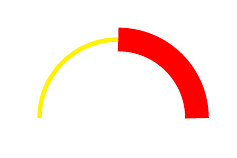
\begin{tikzpicture}
\draw[line width=3mm,red,use Hobby shortcut,save Hobby path={saved}] (0,0) .. ([blank=soft]1,1) .. (2,0);
\draw[ultra thick,yellow,restore and use Hobby path={saved}{disjoint,invert soft blanks}];
\end{tikzpicture}

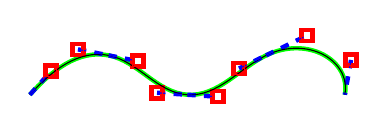
\begin{tikzpicture}[use Hobby shortcut]
\draw[ultra thick,green,postaction=show curve controls]
(0,0) to[save Hobby path={curve},in curl=.1,out curl=3,curve through={(1,.5) .. (2,0) .. (3,.5)}] (4,0);
\begin{scope}%[yshift=-1cm]
\draw[postaction=show curve controls]
(0,0) .. ([in curl=.1,out curl=3]1,.5) .. (2,0) .. (3,.5) .. (4,0);
\end{scope}
\end{tikzpicture}

\tikz[hobby] \draw[save Hobby path={plot}] plot coordinates {(0,0) (1,1) (2,0) (3,1) (2,1) (10:2cm)};


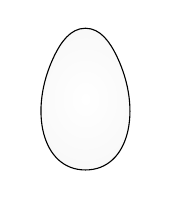
\begin{tikzpicture}[use Hobby shortcut]
\draw[scale=-2,inner color=white,outer color=gray!5] ([closed]0.5,0.1) .. (0.7,0.28) .. (0.5,1) .. (0.3,0.28) .. (0.5,0.1);
\end{tikzpicture}

\newpage

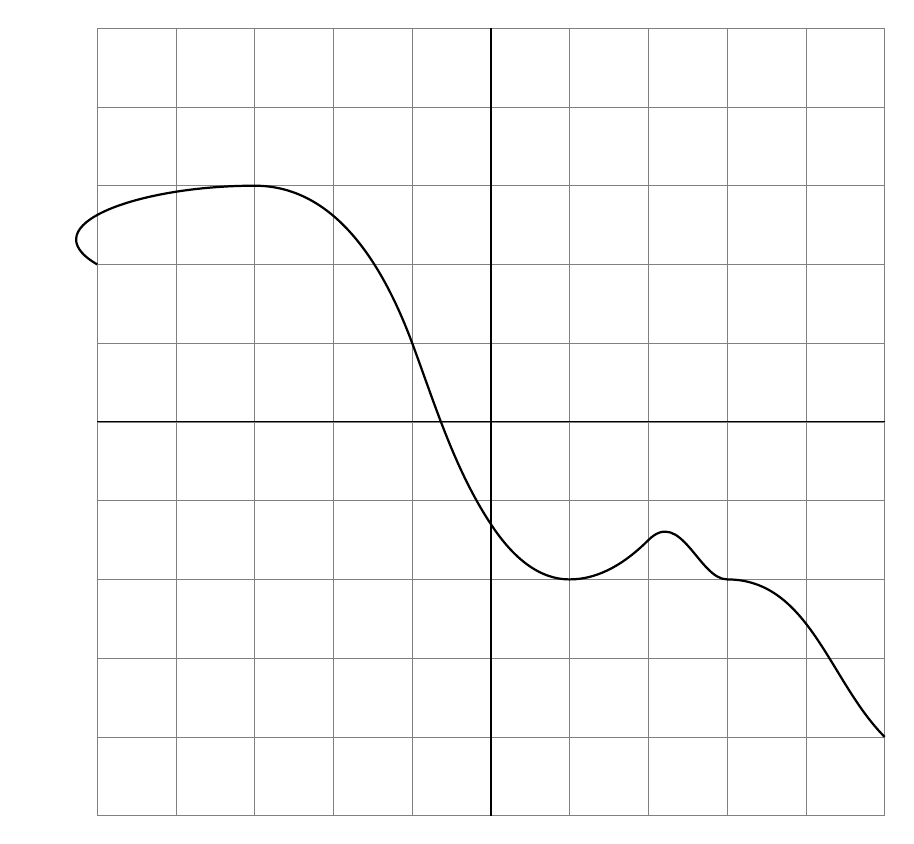
\begin{tikzpicture}[use Hobby shortcut]
\draw[help lines] (-5,-5) grid (5,5);
\draw (-5,0) -- (5,0) (0,-5) -- (0,5);
\draw[thick] ([tangent=150]-5,2) .. ([tangent=0]-3,3) .. (-1,1) .. (0,-1.3) .. ([tangent=0]1,-2) .. ([tangent=45]2,-1.5) .. ([tangent=0]3,-2) .. ([tangent=-45]5,-4);
\end{tikzpicture}

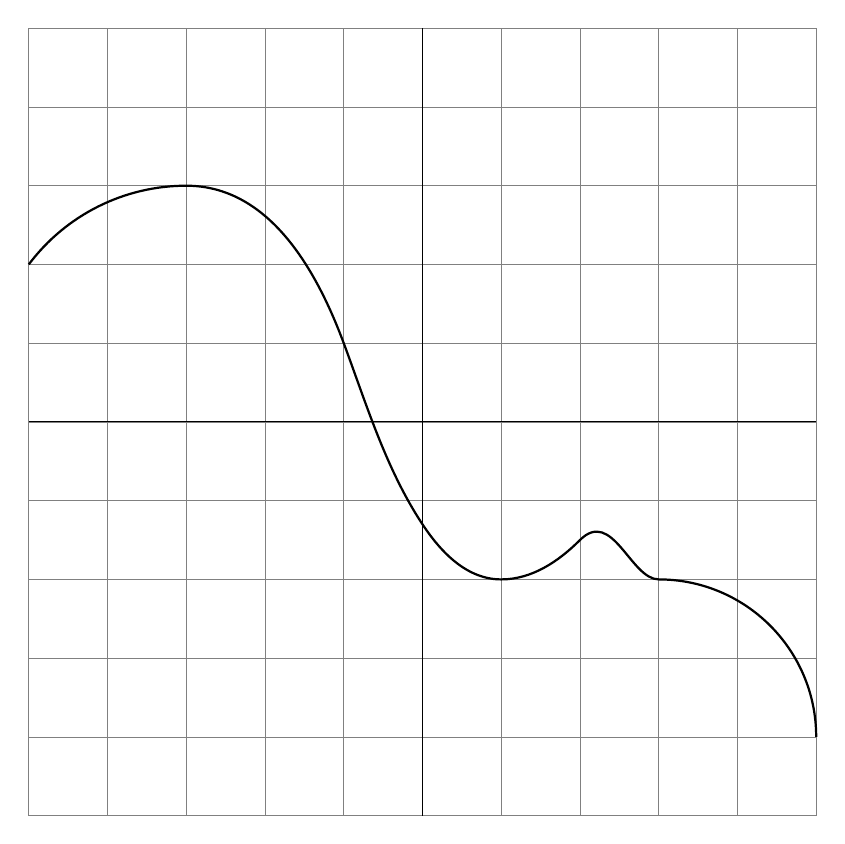
\begin{tikzpicture}[use Hobby shortcut]
\draw[help lines] (-5,-5) grid (5,5);
\draw (-5,0) -- (5,0) (0,-5) -- (0,5);
\draw[thick] (-5,2) .. ([tangent=0]-3,3) .. (-1,1) .. (0,-1.3) .. %
([tangent=0]1,-2) .. ([tangent=45]2,-1.5) .. ([tangent=0]3,-2) .. (5,-4);
\end{tikzpicture}

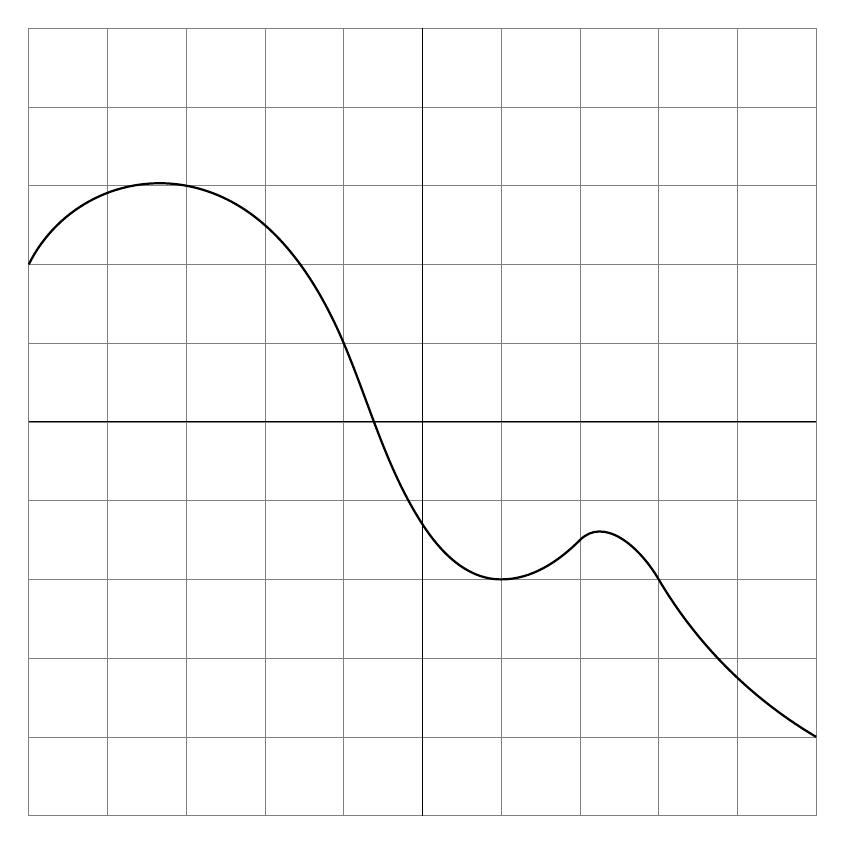
\begin{tikzpicture}[use Hobby shortcut]
\draw[help lines] (-5,-5) grid (5,5);
\draw (-5,0) -- (5,0) (0,-5) -- (0,5);
\draw[thick] (-5,2) .. (-3,3) .. (-1,1) .. (0,-1.3) .. %
([tangent=0]1,-2) .. ([tangent=45]2,-1.5) .. (3,-2) .. (5,-4);
\end{tikzpicture}

\newpage

\begin{tikzpicture}
\draw[use Hobby shortcut] (0,0) .. ([tangent=45]1,1) .. (2,0) .. (3,1) .. (4,0);
\end{tikzpicture}

\begin{tikzpicture}[use Hobby shortcut]
\draw[blue,save Hobby path={left}] ([out angle=90,in angle=-90]1,0) .. (1,1) .. ([blank=soft]0,2) .. (1,3) .. (1,4);
\draw[show Hobby path={left},red] ([out angle=90,in angle=-90]0,0) .. (0,1) .. (1,2) .. (0,3) .. (0,4);
\tikzset{show Hobby path={left}}
\draw[blue,show Hobby path={left},restore and use Hobby path={left}{disjoint,invert soft blanks}];
\end{tikzpicture}

\begin{tikzpicture}[use Hobby shortcut]
\draw[blue,save Hobby path={upper}] ([out angle=0,in angle=-180]0,1) .. (1,1) .. ([blank=soft]2,0) .. (3,1) .. (4,1);
\draw[show Hobby path={upper},red] ([out angle=0,in angle=-180]0,0) .. (1,0) .. (2,1) .. (3,0) .. (4,0);
\tikzset{show Hobby path={upper}}
\draw[blue,show Hobby path={upper},restore and use Hobby path={upper}{disjoint,invert soft blanks}];
\end{tikzpicture}

\begin{tikzpicture}[use Hobby shortcut]
\draw ([out angle=0]0,0) .. (0,2);
\draw ([out angle=0]0,0) .. (2,0);
\begin{scope}[xshift=3cm]
\draw ([out angle=90]0,0) .. (0,2);
\draw ([out angle=90]0,0) .. (2,0);
\begin{scope}[xshift=3cm]
\draw ([out angle=180]0,0) .. (0,2);
%\draw ([out angle=180]0,0) .. (2,0);
\end{scope}
\end{scope}
\end{tikzpicture}


\newpage
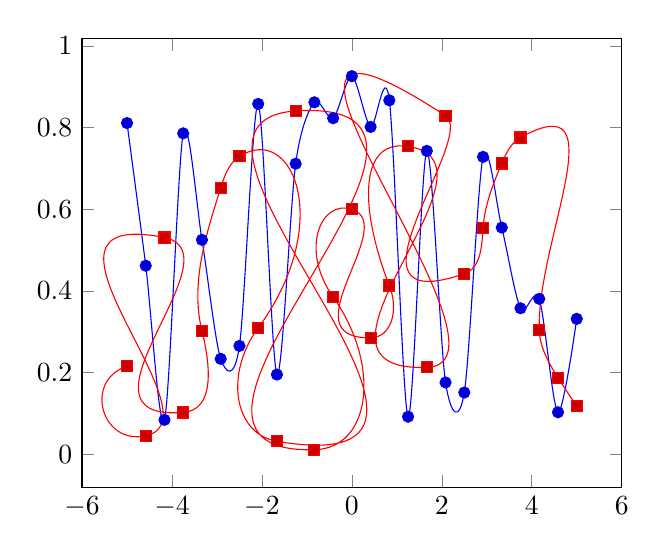
\begin{tikzpicture}
\begin{axis}
\addplot +[smooth] {rnd};
\addplot +[hobby] {rnd};
\end{axis}
\end{tikzpicture}

\newpage



%\tikzset{use quick Hobby shortcut}

\begin{tikzpicture}
\draw[use Hobby shortcut] (0,0) .. (1,1) .. (2,1);
\end{tikzpicture}

\newpage

\tikz[smooth] \draw plot coordinates {(0,0) (1,1) (2,0) (3,1) (2,1) (10:2cm)};

\tikz[hobby] \draw plot coordinates {(0,0) (1,1) (2,0) (3,1) (2,1) (10:2cm)};

\tikz[closed hobby] \draw plot coordinates {(0,0) (1,1) (2,0) (3,1) (2,1) (10:2cm)};

\tikz[quick hobby] \draw plot coordinates {(0,0) (1,1) (2,0) (3,1) (2,1) (10:2cm)};

\newpage

\begin{tikzpicture}[use Hobby shortcut]
\draw ([out angle=10]0,0) .. ([in angle=90]1,1);
\end{tikzpicture}

\begin{tikzpicture}[use Hobby shortcut]
\draw ([out angle=10]0,0) .. ([in angle=90]1,1);
\end{tikzpicture}

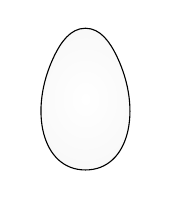
\begin{tikzpicture}[use Hobby shortcut]
\draw[scale=-2,inner color=white,outer color=gray!5] ([closed]0.5,0.1) .. (0.7,0.28) .. (0.5,1) .. (0.3,0.28) .. (0.5,0.1);
\end{tikzpicture}


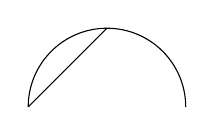
\begin{tikzpicture}[use Hobby shortcut]
\draw (0,0) .. (1,1) .. (2,0);
\draw (0,0) \foreach \k in {1} { .. (\k^2, \k)};
\end{tikzpicture}

\tikz[hobby] \draw plot coordinates {(0,0) ([blank=true]1,1) (2,0) (3,1) (2,1) (10:2cm)};

\tikz[use Hobby shortcut] \draw (0,0) .. (1,1) .. ([blank=true]2,0) .. (3,1) .. ([blank=true]2,1) .. (10:2cm);

\tikz \draw (0,0) to[quick curve through={(1,1) (2,0) ([quick hobby/blank curve=once]3,1) (2,1)}] (10:2cm);

\tikz \draw plot coordinates {(0,0) (1,1) (2,0) (3,1) (2,1) (10:2cm)};

\tikz[smooth] \draw plot coordinates {(0,0) (1,1) (2,0) (3,1) (2,1) (10:2cm)};

\tikz[hobby] \draw (1,0) -- plot coordinates {(0,0) (1,1) (2,0) (3,1) (2,1) (10:2cm)};

\tikz[closed hobby] \draw plot coordinates {(0,0) (1,1) (2,0) (3,1) (2,1) (10:2cm)};

\tikz[quick hobby] \draw plot coordinates {(0,0) (1,1) (2,0) (3,1) (2,1) (10:2cm)};

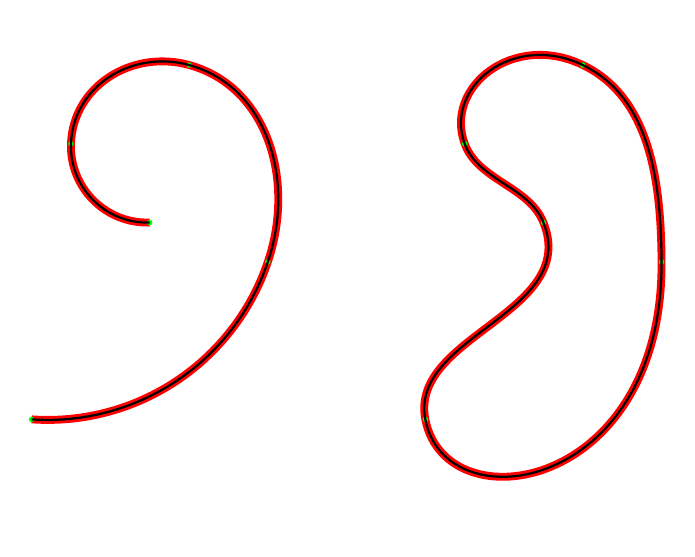
\begin{tikzpicture}[scale=.5]
\draw[scale=.1,line width=1mm,red] (0,0)
.. controls (26.76463,-1.84543) and (51.4094,14.58441) .. (60,40)
.. controls (67.09875,61.00188) and (59.76253,84.57518) .. (40,90)
.. controls (25.35715,94.01947) and (10.48064,84.5022) .. (10,70)
.. controls (9.62895,58.80421) and (18.80421,49.62895) .. (30,50);
\fill[green] (0,0) circle[radius=2pt]
(6,4) circle[radius=2pt]
(4,9) circle[radius=2pt]
(1,7) circle[radius=2pt]
(3,5) circle[radius=2pt];
\draw[thick] (0,0) to[curve through={(6,4) .. (4,9) .. (1,7)}] (3,5);
\begin{scope}[xshift=10cm]
\draw[scale=.1,line width=1mm,red] (0,0)
.. controls (5.18756,-26.8353) and (60.36073,-18.40036) .. (60,40)
.. controls (59.87714,59.889) and (57.33896,81.64203) .. (40,90)
.. controls (22.39987,98.48387) and (4.72404,84.46368) .. (10,70)
.. controls (13.38637,60.7165) and (26.35591,59.1351) .. (30,50)
.. controls (39.19409,26.95198) and (-4.10555,21.23804) .. (0,0); % 
\fill[green] (0,0) circle[radius=2pt]
(6,4) circle[radius=2pt]
(4,9) circle[radius=2pt]
(1,7) circle[radius=2pt]
(3,5) circle[radius=2pt];
\draw[thick] (0,0) to[closed,curve through={(6,4) .. (4,9) .. (1,7)}] (3,5);
\end{scope}
\end{tikzpicture}


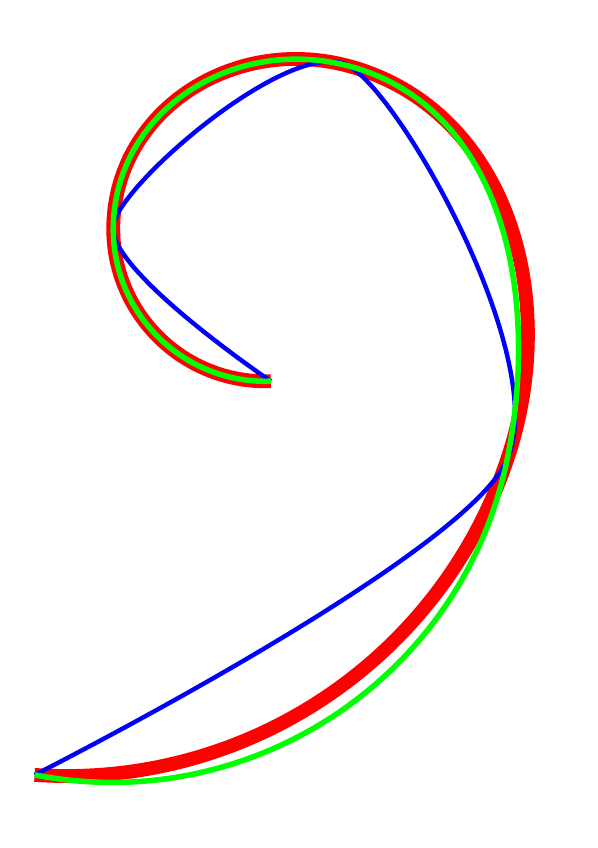
\begin{tikzpicture}
\draw[red,line width=5pt] (0,0) to[curve through={(6,4) .. (4,9) .. (1,7)}] (3,5);
\draw[ultra thick,blue] plot[smooth] coordinates {(0,0) (6,4) (4,9) (1,7) (3,5)};
\draw[green,line width=2pt] (0,0) to[quick curve through={(6,4) (4,9)  (1,7)}] (3,5);
\end{tikzpicture}

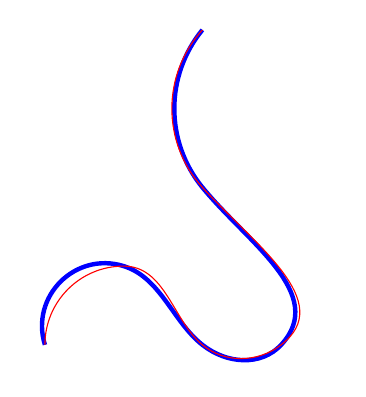
\begin{tikzpicture}[use Hobby shortcut]
\draw[ultra thick,blue] (0,0) .. (1,1) .. (2,0) .. (3,0) .. (2,2) .. (2,4);
\draw[red] (0,0) to[quick curve through={(1,1) (2,0) (3,0) (2,2)}] (2,4);
\end{tikzpicture}

\section{A Piecewise Version of Hobby's Algorithm}

Here we present a variant of Hobby's algorithm.
One difficulty with Hobby's algorithm is that it works with the path as a whole.
It is therefore not possible to build up a path piecewise.
We therefore modify it to correct for this.
Obviously, the resulting path will be less ``ideal'', but will have the property that adding new points will not affect earlier segments.

The method we use is to employ Hobby's algorithm on the two-{}segment subpaths.
This provides two cubic Bezier curves: one from the \(k\)th point to the \(k+1\)st point and the second from the \(k+1\)st to the \(k+2\)nd.
Of this data, we keep the first segment and use that for the path between the \(k\)th and \(k+1\)st points.
We also remember the outgoing angle of the first segment and use that as the incoming angle on the next computation (which will involve the \(k+1\)st, \(k+2\)nd, and \(k+3\)rd) points.

The two ends are slightly different to the middle segments.
On the first segment, we might have no incoming angle.
On the last segment, we render both pieces.

This means that for the initial segment, we have a \(2 \times 2\) linear system:
%
\[
  \begin{bmatrix}
  B_0 & C_0 \\
  A_1 & B_1
  \end{bmatrix}
  \Theta = \begin{bmatrix}
  D_0 \\ D_1
  \end{bmatrix}
\]
%
This has solution:
%
\[
  \Theta = \frac{1}{B_0 B_1 - C_0 A_1} \begin{bmatrix} B_1 & - C_0 \\ -A_1 & B_0 \end{bmatrix} \begin{bmatrix} D_0 \\ D_1 \end{bmatrix} =  \frac{1}{B_0 B_1 - C_0 A_1} \begin{bmatrix} B_1 D_0 - C_0 D_1 \\ B_0 D_1 - A_1 D_0 \end{bmatrix}
\]

Now we have the following values for the constants:
%
\begin{align*}
A_1 &= d_1 \overline{\tau}_2 \overline{\tau}_1^2 \\
%
B_0 &= \tau_0^3 (3 \overline{\tau}_1 - 1) + \chi_0 \overline{\tau}_1^3 \\
%
B_1 &= d_1 \overline{\tau}_2 \overline{\tau}_1^2 (3 \tau_0 - 1) + d_0 \tau_0 \tau_1^2(3 \overline{\tau}_2 - 1) - d_0 \tau_0 \tau_1^2 \frac{\overline{\tau}_2^3 + \chi_2 \tau_1^3 (3 \overline{\tau}_2 - 1)}{\overline{\tau}_2^3 (3 \tau_1 - 1) + \chi_2 \tau_1^3} \\
%
C_0 &= \tau_0^3 + \chi_0 \overline{\tau}_1^3 (3 \tau_0 - 1) \\
%
D_0 &= - (\tau_0^3 + \chi_0 \overline{\tau}_1^3 ( 3 \tau_0 - 1)) \psi_1 \\
%
D_1 &= - d_1 \overline{\tau}_2 \overline{\tau}_1^2 (3 \tau_0 - 1) \psi_1
\end{align*}
%

Let us, for simplicity at the start, assume that the tensions and curls are all \(1\).
Then we have \(A_1 = d_1\), \(B_0 = 3\), \(B_1 = 2 d_1 + 2 d_0 - d_0 = 2 d_1 + d_0\), \(C_0 = 3\), \(D_0 = - 3 \psi_1\), \(D_1 = - 2 d_1 \psi_1\).
Thus the linear system is:
%
\[
  \begin{bmatrix}
  3 & 3 \\
  d_1 & 2 d_1 + d_0
  \end{bmatrix}
  \Theta = - \psi_1 \begin{bmatrix}
  3 \\ 2 d_1
  \end{bmatrix}
\]
%
which we can row reduce to:
%
\[
  \begin{bmatrix}
  1 & 1 \\
  0 & d_1 + d_0 
  \end{bmatrix}
  \Theta = -\psi_1 \begin{bmatrix}
  1 \\ d_1
  \end{bmatrix}
\]
%
whence \(\theta_1 = -\psi_1 \frac{d_1}{d_0 + d_1}\) and \(\theta_0 = -\psi_1 - \theta_1 = -\psi_1\frac{d_0 }{d_0 + d_1}\).
We also compute \(\phi_1 = -\psi_1 - \theta_1 = \theta_0\) and \(\phi_2 = \theta_1\) (in the simple version).
We use \(\theta_0\) and \(\phi_1\) to compute the bezier curve of the first segment, make a note of \(\theta_1\), and -- assuming there are more segments -- throw away \(\phi_2\).

For the inner segments, we have the system:
%
\[
  \begin{bmatrix}
  1 & 0 \\
  A_1 & B_1
  \end{bmatrix}
  \Theta = \begin{bmatrix}
  \theta_0 \\
  D_1
  \end{bmatrix}
\]
%
which has the solution \(\theta_1 = (D_1 - A_1 \theta_0)/B_1\).
The values of the constants in this case are:
%
\begin{align*}
A_1 &= d_1 \overline{\tau}_2 \overline{\tau}_1^2 \\
%
B_1 &= d_1 \overline{\tau}_2 \overline{\tau}_1^2 (3 \tau_0 - 1) + d_0 \tau_0 \tau_1^2(3 \overline{\tau}_2 - 1) - d_0 \tau_0 \tau_1^2 \frac{\overline{\tau}_2^3 + \chi_2 \tau_1^3 (3 \overline{\tau}_2 - 1)}{\overline{\tau}_2^3 (3 \tau_1 - 1) + \chi_2 \tau_1^3} \\
%
D_1 &= - d_1 \overline{\tau}_2 \overline{\tau}_1^2 (3 \tau_0 - 1) \psi_1
\end{align*}

Again, let us consider the simpler case.
Then \(A_1 = d_1\), \(B_1 = 2 d_1 + d_0\), and \(D_1 = - 2 d_1 \psi_1\).
Thus \(\theta_1 = (-2 d_1 \psi_1 - d_1 \theta_0)/(2 d_1 + d_0) = - (2 \psi_1 + \theta_0) \frac{d_1}{2 d_1 + d_0}\).
We compute \(\phi_1 = -\psi_1 - \theta_1 = \frac{- \psi_1 d_0 + \theta_0 d_1}{2 d_1 + d_0}\) and \(\phi_2 = \theta_1\).

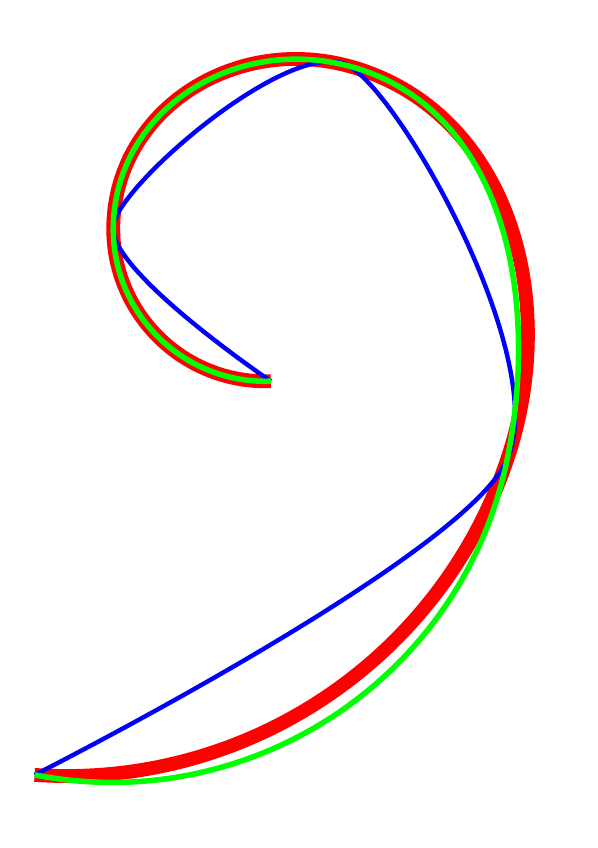
\begin{tikzpicture}
\draw[red,line width=5pt] (0,0) to[curve through={(6,4) .. (4,9) .. (1,7)}] (3,5);
\draw[ultra thick,blue] plot[smooth] coordinates {(0,0) (6,4) (4,9) (1,7) (3,5)};
\draw[green,line width=2pt] (0,0) to[quick curve through={(6,4) (4,9)  (1,7)}] (3,5);
\end{tikzpicture}


\begin{tikzpicture}[use Hobby shortcut, c/.style={insert path={circle[radius=2pt]}}]
\fill[green] (0,0) [c] (1,.5) [c] (0,0) [c] (3,.5) [c] (4,0) [c];
\draw (0,0) .. (1,.5) .. (-0.2,0) .. (3,.5) .. (4,0);
\end{tikzpicture}

\begin{tikzpicture}
\draw (0.0000, 0.0000) .. controls (-1.85420, 0.83131) and (1.44747, 2.48215)..(1.0000, 0.5000) .. controls (0.90917, 0.09765) and (0.31923, 0.27721)..(0.1000, 0.0000) .. controls (-1.10155, -1.51937) and (1.46789, -0.02595)..(3.0000, 0.5000) .. controls (3.41450, 0.64229) and (3.86513, 0.41698)..(4.0000, 0.0000);
\end{tikzpicture}

\begin{tikzpicture}
\draw (0.0000, 0.0000) .. controls (0.30056, -0.75821) and (1.42623, -0.19537)..(1.0000, 0.5000) .. controls (0.69595, 0.99605) and (-0.14029, 0.67496)..(0.0000, 0.0000) .. controls (0.31344, -1.50803) and (1.85232, 0.35331)..(3.0000, 0.5000) .. controls (3.40390, 0.55162) and (3.79896, 0.35409)..(4.0000, 0.0000);
\end{tikzpicture}

\begin{tikzpicture}
\draw (0,0) to[curve through={(6,4) .. (4,9) .. (1,7)}] (3,5);
\end{tikzpicture}

\begin{tikzpicture}
\draw (0,0) to[closed,curve through={(6,4) .. (4,9) .. (1,7)}] (3,5);
\end{tikzpicture}
\end{document}


% Local Variables:
% tex-output-type: "pdf18"
% End:
